\documentclass[conference]{IEEEtran}

\usepackage{amsmath,amssymb}
\usepackage{graphicx}
\usepackage{booktabs}
\usepackage{cite}
\usepackage{hyperref}

\graphicspath{{../../../phase_01_python_prototype/figures/}}

\title{Lightweight Spike-Based DOA Sector Classification for Embedded Edge Inference}

\author{\IEEEauthorblockN{Hossein Molhem}
\IEEEauthorblockA{Department of Electrical and Computer Engineering\\
Kennesaw State University\\
Email: hmolhem@students.kennesaw.edu}}

\begin{document}
\maketitle

\begin{abstract}
This paper presents a compact Python reference prototype for direction-of-arrival (DOA) sector classification using a physics-based uniform linear array (ULA) signal model and a leaky-integrate-and-fire (LIF)-inspired inference path. The objective is not to introduce a new DOA estimator, but to establish a reproducible embedded-AI baseline that connects array signal processing, sparse spike encoding, and latency-aware temporal inference. Beamspace energy features are extracted from sample covariance matrices and classified using both a nearest-centroid non-spiking baseline and a rate-coded LIF-inspired classifier. The nearest-centroid baseline achieves an overall accuracy of 86.90\%. A fixed LIF configuration achieves 82.50\% accuracy, while a time-window/leak parameter sweep improves the best LIF accuracy to 84.17\%. The results show a clear accuracy--latency trade-off suitable for later embedded implementation studies.
\end{abstract}

\begin{IEEEkeywords}
Embedded AI, spiking neural networks, LIF neuron, DOA classification, uniform linear array, edge inference, beamspace features.
\end{IEEEkeywords}

\section{Introduction}

Edge sensing systems often require inference under constrained compute, memory, and latency budgets. For such systems, lightweight and hardware-aware inference methods can be preferable to large black-box neural networks. Spike-based inference is attractive because information can be represented through sparse temporal events, potentially reducing arithmetic activity and supporting early decision logic.

This work uses DOA sector classification as a controlled sensing problem. The selected problem is technically relevant because it is grounded in array signal processing, yet compact enough to support an end-to-end Phase 1 prototype. The contribution is an engineering baseline that compares continuous-valued beamspace classification with a sparse LIF-inspired temporal inference path.

\section{Signal Model}

A narrowband single-source ULA model is used. For source angle $\theta$, the received snapshot matrix is
\begin{equation}
    X = a(\theta)s + N,
\end{equation}
where $a(\theta)$ is the steering vector, $s$ is the source signal, and $N$ is circular complex Gaussian noise. The sample covariance matrix is
\begin{equation}
    R_{xx}=\frac{1}{M}XX^{H},
\end{equation}
where $M=128$ snapshots.

Beamspace energy features are extracted over a fixed angular grid. The classification target is not the exact continuous angle, but one of four coarse angular sectors spanning $-60^{\circ}$ to $+60^{\circ}$.

\section{Methodology}

\subsection{Dataset Configuration}

\begin{table}[t]
\centering
\caption{Dataset Configuration}
\begin{tabular}{ll}
\toprule
Parameter & Value \\
\midrule
Array elements & 8 \\
Snapshots & 128 \\
Spacing & $\lambda/2$ \\
DOA range & $-60^{\circ}$ to $+60^{\circ}$ \\
Sectors & 4 \\
SNR values & $-10$ to $20$ dB \\
Total samples & 2800 \\
Test samples & 840 \\
\bottomrule
\end{tabular}
\end{table}

The dataset contains 100 samples per sector per SNR value. A 70/30 train/test split is used with stratification by SNR and class.

\subsection{Nearest-Centroid Baseline}

The baseline classifier is a nearest-centroid classifier applied to normalized beamspace feature vectors. This classifier is deterministic and interpretable, making it an appropriate reference point for measuring the effect of spike encoding.

\subsection{Rate-Based Spike Encoding}

Normalized features are converted into binary spike trains using rate-based encoding. Higher normalized feature values correspond to higher spike probabilities over a finite time window.

\subsection{LIF-Inspired Classifier}

The LIF-inspired classifier is implemented as a leaky membrane accumulator for each class:
\begin{equation}
    v_c[t]=\alpha v_c[t-1]+i_c[t],
\end{equation}
where $v_c[t]$ is the class membrane state, $\alpha$ is the leak factor, and $i_c[t]$ is the spike-driven input current. The class with the largest final membrane value is selected. Stable-decision latency is estimated as the earliest time after which the final decision remains unchanged.

\section{Results}

The nearest-centroid baseline achieved an overall accuracy of 0.869048. The fixed LIF configuration with $T=20$ and leak $=0.97$ achieved 0.825000 accuracy and a mean stable-decision latency of 6.423810 time steps.

\begin{figure}[t]
\centering
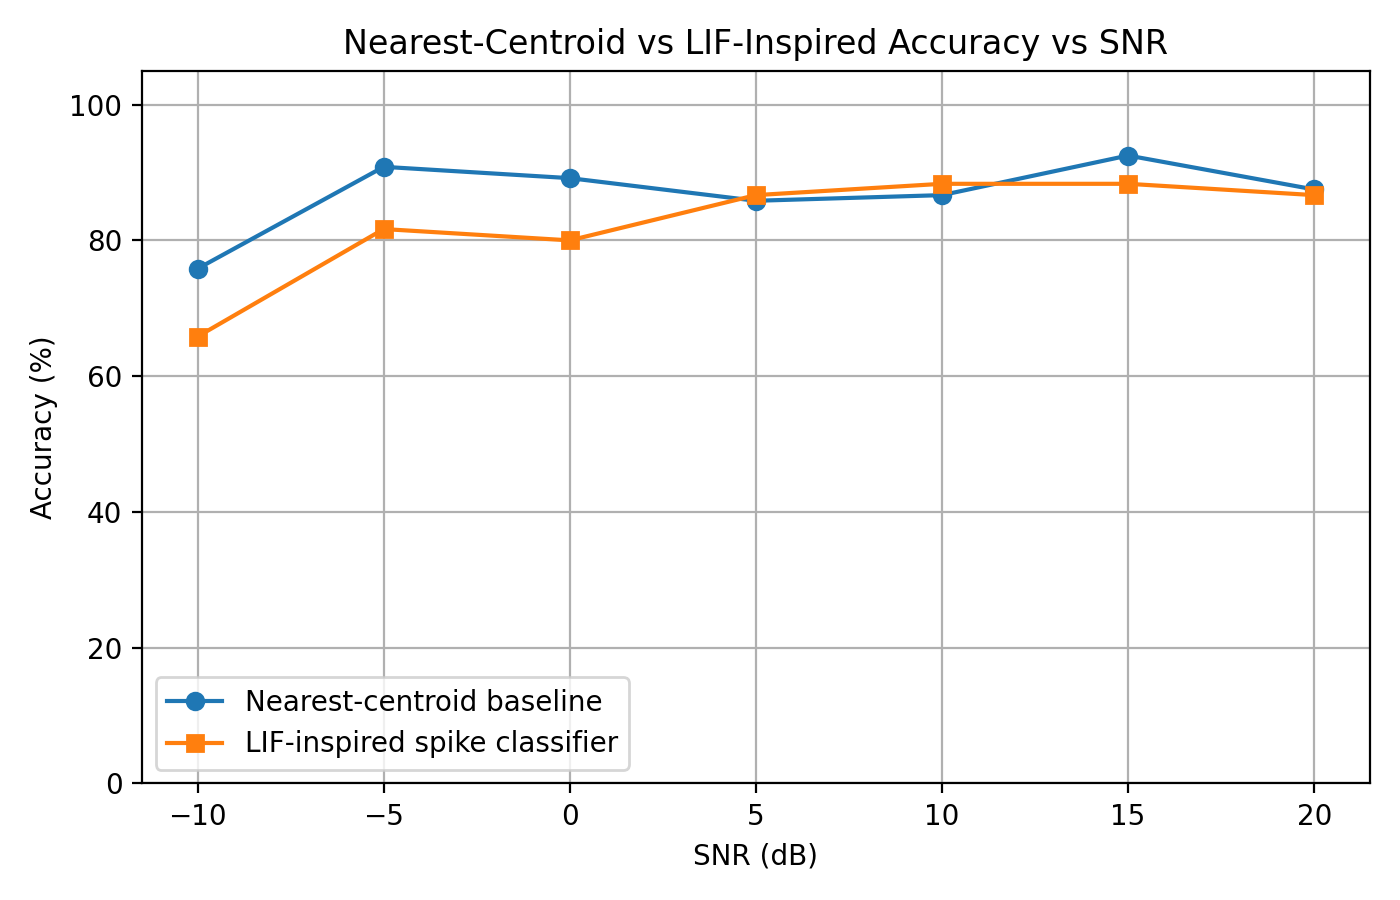
\includegraphics[width=0.95\linewidth]{run_004_accuracy_comparison_vs_snr.png}
\caption{Accuracy comparison between the nearest-centroid baseline and the fixed LIF-inspired classifier.}
\label{fig:accuracy}
\end{figure}

\begin{figure}[t]
\centering
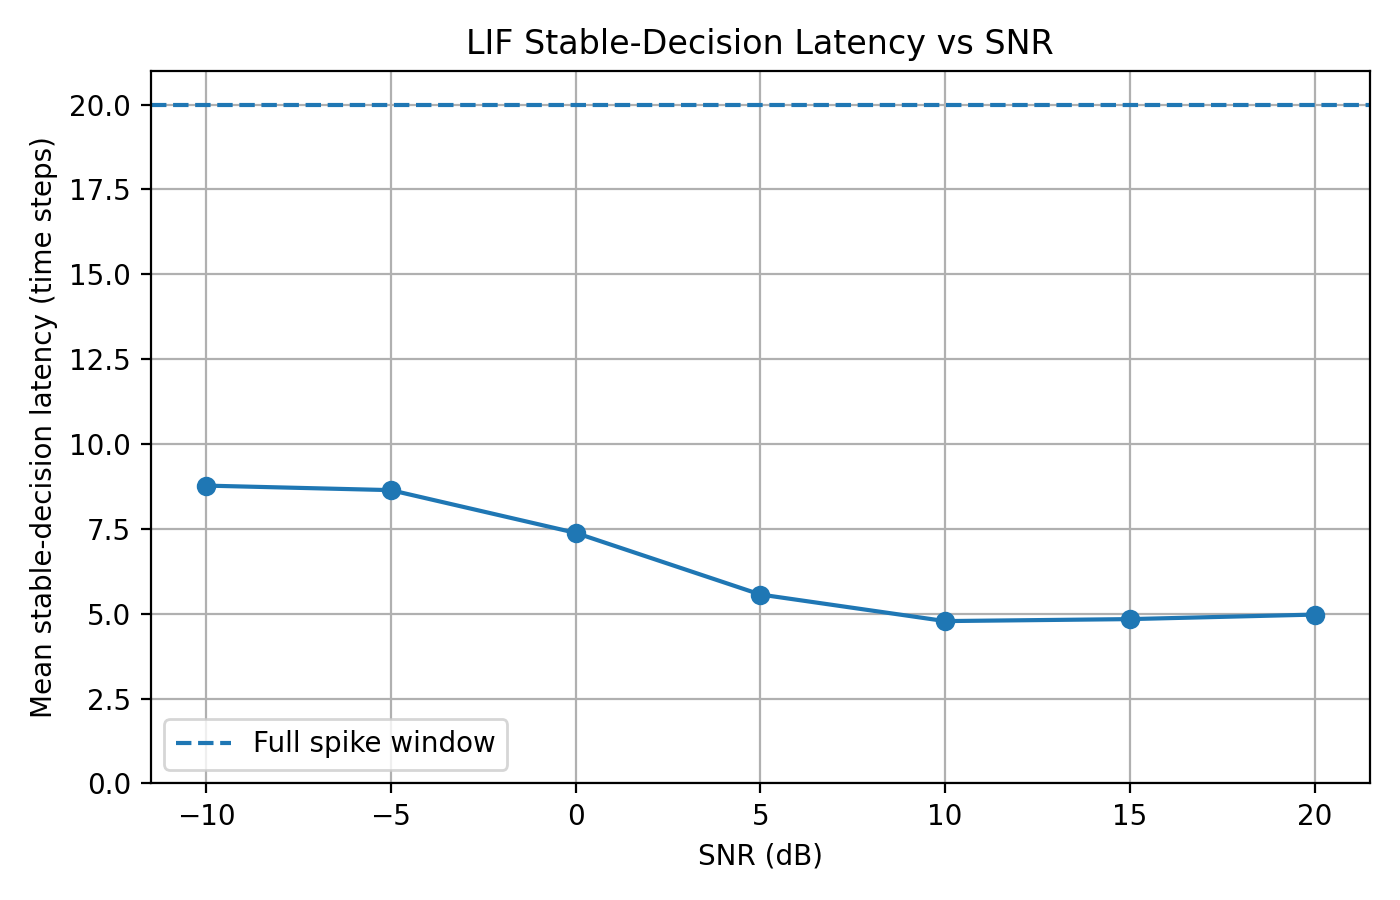
\includegraphics[width=0.95\linewidth]{run_004_lif_latency_vs_snr.png}
\caption{Mean stable-decision latency versus SNR for the LIF-inspired classifier.}
\label{fig:latency}
\end{figure}

Run 005 swept the number of time steps and membrane leak factor. Table~\ref{tab:sweep} summarizes the most important cases.

\begin{table}[t]
\centering
\caption{Key Run 005 Sweep Results}
\label{tab:sweep}
\begin{tabular}{lrrrr}
\toprule
Case & $T$ & Leak & Acc. & Lat. \\
\midrule
Best LIF accuracy & 40 & 0.99 & 0.841667 & 8.396429 \\
Lowest latency & 10 & 0.99 & 0.776190 & 3.782143 \\
Fixed reference & 20 & 0.97 & 0.825000 & 6.423810 \\
Baseline & -- & -- & 0.869048 & -- \\
\bottomrule
\end{tabular}
\end{table}

\begin{figure}[t]
\centering
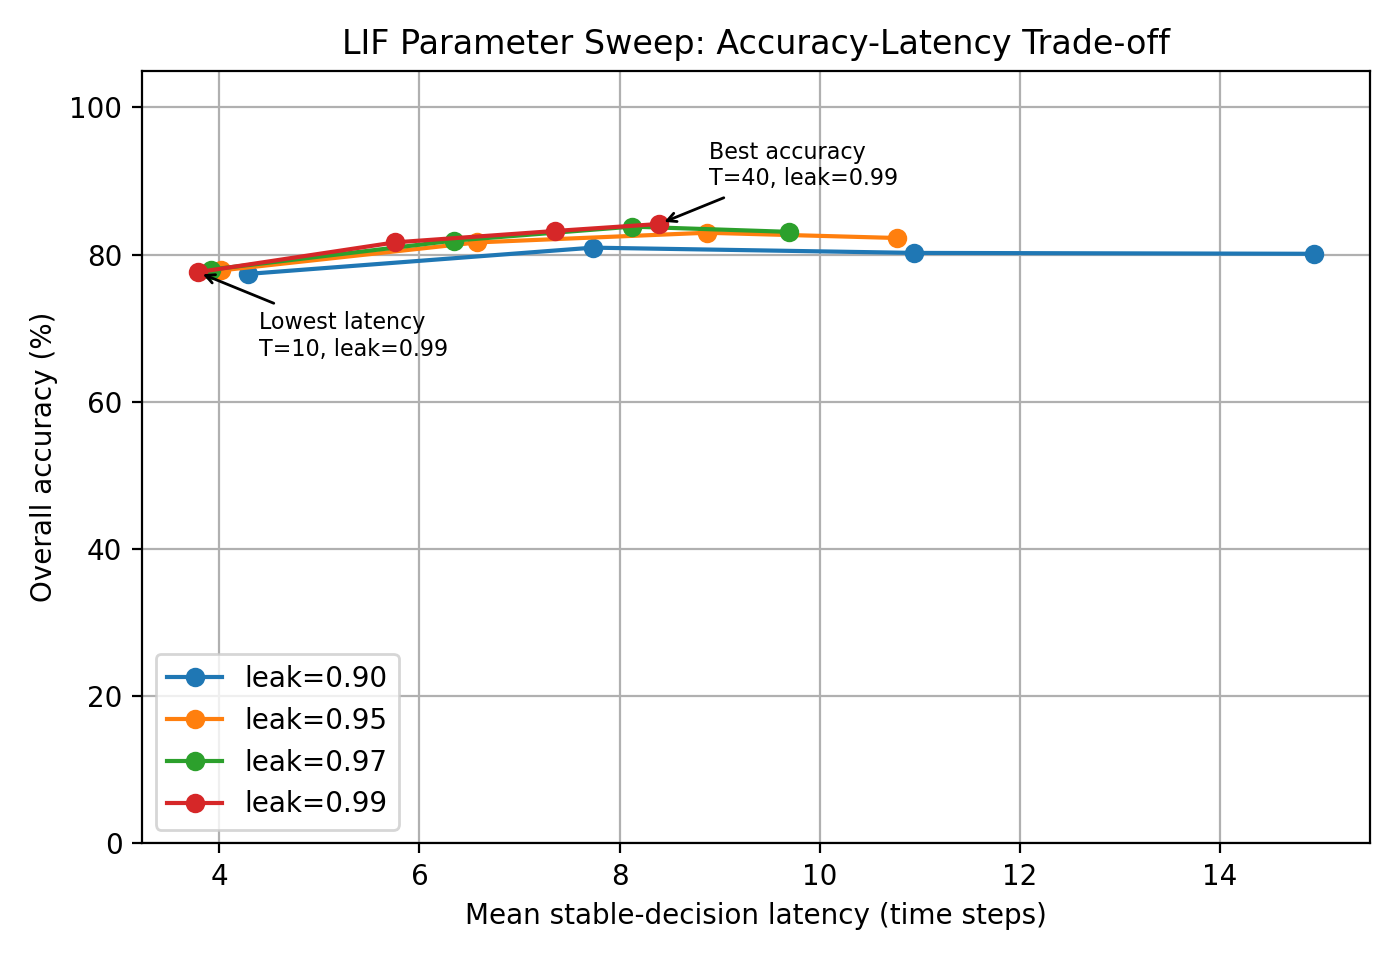
\includegraphics[width=0.95\linewidth]{run_005_lif_accuracy_latency_tradeoff.png}
\caption{Accuracy--latency trade-off for the LIF time-window and leak sweep.}
\label{fig:tradeoff}
\end{figure}

\section{Discussion}

The results show that compact beamspace features are informative for sector-level DOA classification. The non-spiking nearest-centroid classifier achieves the highest accuracy, as expected, because it operates directly on continuous-valued normalized features. The LIF-inspired classifier incurs some accuracy loss because the features are converted into sparse stochastic spike trains. However, this loss is moderate, and the LIF path provides a tunable temporal decision process.

The parameter sweep confirms that longer time windows generally improve accuracy, while shorter time windows reduce mean stable-decision latency. Higher leak values preserve evidence more effectively in this prototype. This behavior is useful for embedded inference because it exposes a design knob between accuracy and latency.

\section{Conclusion}

A complete Phase 1 Python prototype was developed for spike-based DOA sector classification. The system uses a physics-based ULA model, beamspace features, nearest-centroid baseline classification, rate-coded spike trains, and LIF-inspired temporal inference. The best LIF configuration reached 84.17\% accuracy, compared with 86.90\% for the non-spiking baseline. The result establishes a reproducible embedded-AI reference path for later work involving richer radar/DOA cases, PYNQ deployment, and FPGA-oriented acceleration.

\begin{thebibliography}{9}
\bibitem{vantrees}
H. L. Van Trees, \emph{Optimum Array Processing}. Wiley, 2002.

\bibitem{haykin}
S. Haykin, \emph{Adaptive Filter Theory}. Pearson, 2014.

\bibitem{maass}
W. Maass, ``Networks of spiking neurons: The third generation of neural network models,'' \emph{Neural Networks}, vol. 10, no. 9, pp. 1659--1671, 1997.

\bibitem{roy}
K. Roy, A. Jaiswal, and P. Panda, ``Towards spike-based machine intelligence with neuromorphic computing,'' \emph{Nature}, vol. 575, pp. 607--617, 2019.
\end{thebibliography}

\end{document}
